\section{取整函数}
\begin{definition}[取整函数]
设\(x \in \mathbb{R}\),定义:
\begin{enumerate}
	\item 向下取整函数\(\floor{x}\)为不大于\(x\)的最大整数;
	\item 向上取整函数\(\ceil{x}\)为不小于\(x\)的最小整数.
\end{enumerate}
\end{definition}

\begin{figure}[ht]
\def\subwidth{.45\linewidth}
\def\subscale{.9}
\begin{subfigure}[b]{\subwidth}%
\centering
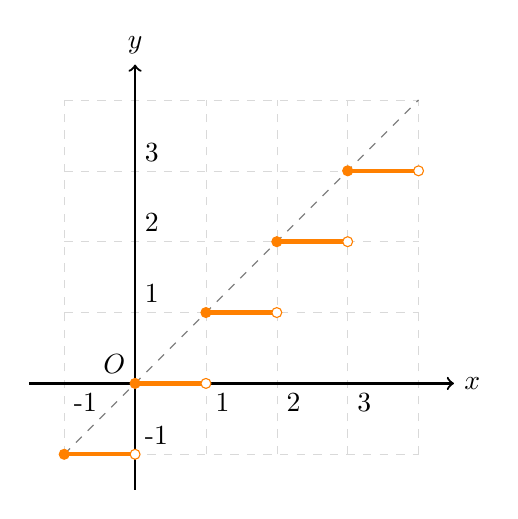
\begin{tikzpicture}[scale=\subscale]
	\tikzstyle{sx}=[draw=orange,fill=orange]
	\tikzstyle{kx}=[draw=orange,fill=white]
	\draw[help lines, color=gray!30, dashed] (-1,-1) grid (4,4);
	\draw[dashed, color=gray] (-1,-1) -- (4,4);
	\draw[->, thick] (-1.5,0) -- (4.5,0) node[right]{\(x\)};
	\draw[->, thick] (0,-1.5) -- (0,4.5) node[above]{\(y\)};
	\foreach \i in {-1,...,3} {
		\draw[ultra thick,orange] (\i,\i)--(\i+1,\i);
		\fill[sx] (\i,\i)circle(2pt);
		\fill[kx] (\i+1,\i)circle(2pt);
		\ifnum\i=0\relax\else
			\draw(\i,0)node[below right]{\i};
			\draw(0,\i)node[above right]{\i};
		\fi
	}
	\draw (0,0)node[above left]{\(O\)};
\end{tikzpicture}
\subcaption{向下取整函数\(\floor{x}\)}
\end{subfigure}
\begin{subfigure}[b]{\subwidth}%
\centering
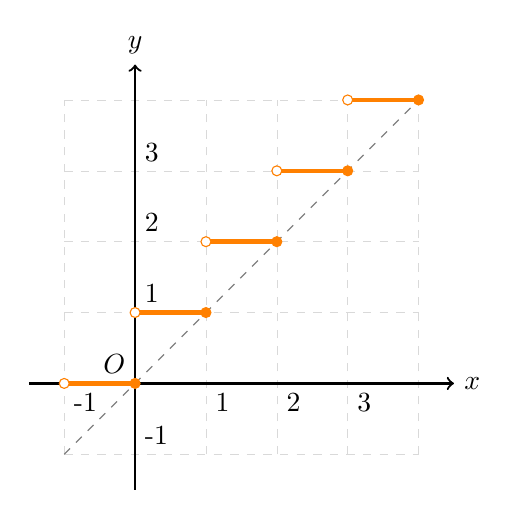
\begin{tikzpicture}[scale=\subscale]
	\tikzstyle{sx}=[draw=orange,fill=orange]
	\tikzstyle{kx}=[draw=orange,fill=white]
	\draw[help lines, color=gray!30, dashed] (-1,-1) grid (4,4);
	\draw[dashed, color=gray] (-1,-1) -- (4,4);
	\draw[->, thick] (-1.5,0) -- (4.5,0) node[right]{\(x\)};
	\draw[->, thick] (0,-1.5) -- (0,4.5) node[above]{\(y\)};
	\foreach \i in {-1,...,3} {
		\draw[ultra thick,orange] (\i,\i+1)--(\i+1,\i+1);
		\fill[kx] (\i,\i+1)circle(2pt);
		\fill[sx] (\i+1,\i+1)circle(2pt);
		\ifnum\i=0\relax\else
			\draw(\i,0)node[below right]{\i};
			\draw(0,\i)node[above right]{\i};
		\fi
	}
	\draw (0,0)node[above left]{\(O\)};
\end{tikzpicture}
\subcaption{向上取整函数\(\ceil{x}\)}
\end{subfigure}
\caption{取整函数的图形}
\end{figure}

\begin{property}
一般地,对于\(x\in\mathbb{R}\),总有\begin{equation}
x - 1 < \floor{x} \leq x \leq \ceil{x} < x + 1.
\end{equation}
\end{property}

\begin{property}
对于\(x\in\mathbb{Z}\),总有\begin{equation}
\ceil{n/2} + \floor{n/2} = n.
\end{equation}
\end{property}

\begin{property}
对于任意实数\(x \geq 0\)和整数\(a,b>0\),总有\begin{gather}
\ceil*{\frac{\ceil{x/a}}{b}} = \ceil*{\frac{x}{ab}}, \\
\floor*{\frac{\floor{x/a}}{b}} = \floor*{\frac{x}{ab}}, \\
\ceil*{\frac{a}{b}} \leq \frac{a+(b-1)}{b}, \\
\floor*{\frac{a}{b}} \geq \frac{a-(b-1)}{b}.
\end{gather}
\end{property}
